\documentclass[12pt, letterpaper, twocolumn]{article}
\usepackage[margin=1.0in]{geometry}
\usepackage{graphicx}
\usepackage{float}
\usepackage{amsmath}
\usepackage{booktabs}
\usepackage{multirow}
\usepackage{tabularx,siunitx}
\usepackage[skip=0.5\baselineskip]{caption}
\usepackage{newtxtext,newtxmath}
\newcommand\mX[1]{\multicolumn{1}{X}{#1}}  % handy shortcut macros
\newcommand\mcc[1]{\multicolumn{2}{c}{#1}}
\newcommand\mcl[1]{\multicolumn{2}{l}{#1}}
\setlength{\headheight}{14.5pt}
\title{Geometric Modeling of Gamma Coincidence}
\author{Austin Smith, Jordan Sturdivant, and Rahul Mehta\\
Department of Physics \& Astronomy, University of Central Arkansas
}
\date{}
\begin{document}
\maketitle{}
% Introduction
\section{Introduction}
A common nuclear process seen in radioactive sources involves the emission of
two gamma rays in coincidence (simultaneously). A source that undergoes this
phenomenon frequently is \textsuperscript{22}Na. \textsuperscript{22}Na exhibits
this process through $\beta$+ decay producing a positronium (positron electron
pair) which annihilates, emitting two gamma rays. These gamma rays in theory
have equal energies of 511 keV and a net momentum that is conserved. The
momentum of the positronium on paper is zero, therefore the direction of each
photon should be 180 degrees from the other to conserve momentum. The goal of
this experiment is too prove the angular correlation between these two
coincident gammas.
% Methods
\section{Method}
The angle of correlation between the coincident gammas, in theory is 180
degrees. This experiment tested this theory through comparing two different
models: the amount of coincidence counted at a given off-set (measured from
180 degrees) angle and a theoretical geometric model of coincident gammas with
180 degree correlation. \setlength{\parskip}{6pt} The general design of the
experiment involved two gamma-ray detectors in a time-gate circuitry wired to
only measure gammas that hit both detectors within a short period of time
between the other (Figure \ref{figure:circuit}). These detectors were set
equidistant (varied from 15 cm to 30 cm) from a source of \textsuperscript{22}NA
where one detector was held still, while the other was rotated freely around the
source (Figure \ref{figure:set_up}).
\begin{figure}[H]
    \centering
    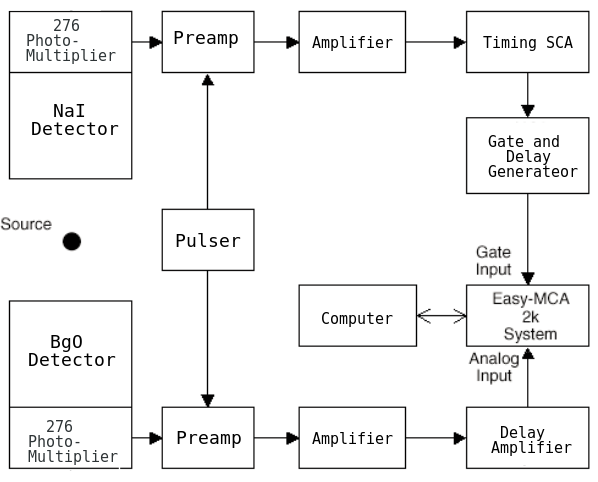
\includegraphics[width=0.45\linewidth]{Figures/gamma_coin_circuitry.png}
    \caption{Circuitry behind the detectors used to measure gamma coincidence.}
    \label{figure:circuit}
    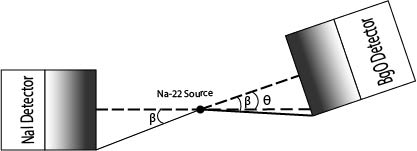
\includegraphics[width=0.45\linewidth]{Figures/detector_set_up.jpg}
    \caption{Set up of angular variation between the two detectors and the
    \textsuperscript{22}Na source.}
    \label{figure:set_up}
\end{figure}
For the first model the angle of the detector was varied in increments of 1-2
degrees offset from 180 and a spectrum of coincident gamma rays was collected
for 120-240 second at each angle. This spectrum was integrated for each angle
to get the desired net count rate (Figure \ref{figure:spectrum}.
\begin{figure}[H]
    \centering
    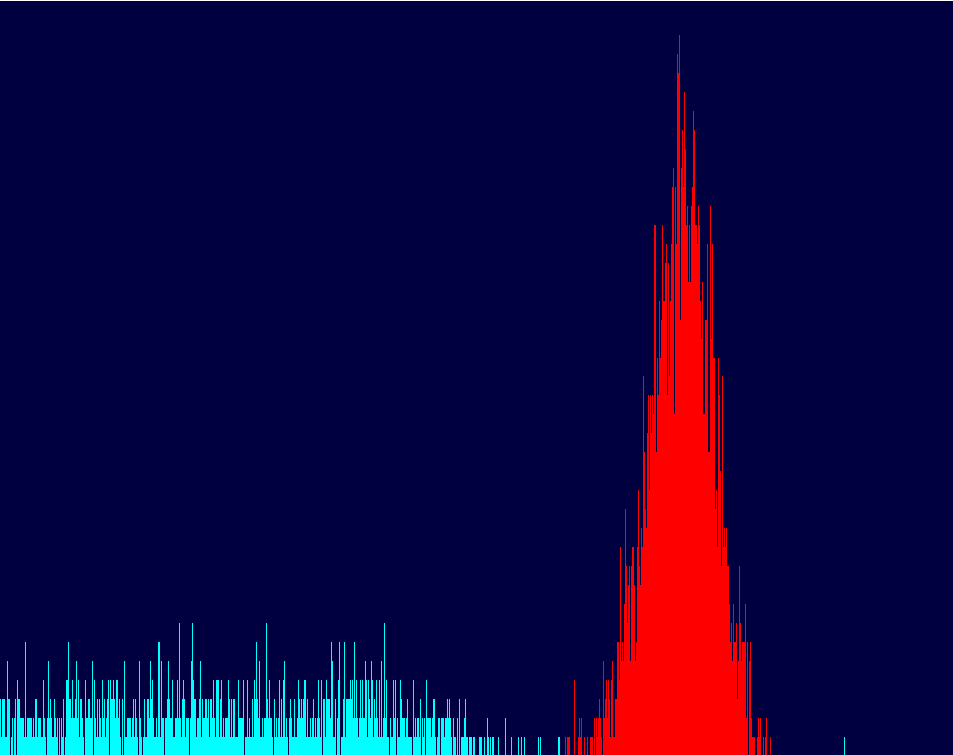
\includegraphics[width=0.45\linewidth]{Figures/sample_spectrum.png}
    \caption{Spectrum produced with the detectors 15 cm and 0 degrees offset
    from the source. Peak highlighted was integrated for count rate.}
    \label{figure:spectrum}
\end{figure}
The second model aims to compares the overlapping area between detectors with
the net count rate per angle. If coincident gammas eject directly opposite from
each other, in order for any coincidence to be measured, part of the face of
each
detector must overlap the other. This is essentially a measure of the set-ups
ability to count coincidence and the general trend can be compared with the
first set of data to see if the theory is supported.
% Results
\section{Results}
Table 1 \& 2 measured count rates at their respective offset angle from 180
degrees. The trend turned out to be similar for both distances from the source
showing a maximum count rate somewhere between -1 to 1 degrees, and following a
Gaussian curve as the offset angle increased from the 180 degree angle.
(Figure \ref{figure:model1_graph}). \setlength{\parskip}{6pt} For the second
model the overlapping area of the detectors was solved as a function of offset
angle using the geometry displayed in Figure \ref{figure:geometry}. These
geometric correlations allow the area of overlap to be expressed only in terms
of angle and the fixed detector radius'. To start this derivation, we found the
total area overlapped to be a linear combination of the area of the two inner
circles $A_{1}$ \& $A_{2}$ as labeled in Figure \ref{figure:geometry}. The areas
of these pieces follow as:
\begin{equation}
  \begin{gathered}
   A_{1} = 2\int_{d1}^{r1}\sqrt{r_{1}^{2}-x^{2}}dx \nonumber\\
   A_{2} = 2\int_{d-r_{2}}^{d1}\sqrt{r_{2}^{2}-(x-d)^{2}}dx \nonumber
  \end{gathered}
\end{equation}
After substitution and simplification we are left with:
\begin{equation}
  \begin{aligned}
  A_{total}=r_{1}^{2}cos^{-1}(\frac{d_{1}}{r_{1}})−d_{1}\sqrt{r_{1}^{2}−d_{1}^
  {2}}\\+r_{2}^{2}cos^{-1}(\frac{d_{2}}{r_{2}})−d_{2}\sqrt{r_{2}^{2}−d_{2}^{2}}
  \nonumber
  \end{aligned}
\end{equation}
where...
\begin{equation}
  \begin{aligned}
  d_{1} = \frac{r_{1}^{2}-r_{2}^{2}+d^{2}}{2d} \nonumber \\ d_{2} =
  \frac{r_{2}^{2}-r_{1}^{2}+d^{2}}{2d} \nonumber \\ d = \imath \cdot sin(\theta)
  \end{aligned}
\end{equation}
This formula only holds true for when $r_{1}\geq r_{2}$ and $d \geq r_{2} -
r_{1}$. Assertion 1 is always true in our set-up, however due to Assertion 2,
the correlation falls apart when the offset angle from 180 degrees is small.
These points were removed from the data. Once all of the overlapping areas were
calculate, we plotted and attempted to fit the data. When fit, the data didn't
correspond to any common model well, however the general trend still shows a
maximum at 0 degrees, and a steep decrease in area as the angle sweeps in
either direction from this maximum (Figure \ref{figure:model2_graph}).
\begin{table}[H]
\centering
\begin{tabular}{ccccc}
\toprule
{Angles} & \multicolumn{4}{c}{Distance}\\\cmidrule{2-5}
& \mcc{\textbf{15 cm}}
& \mcc{\textbf{30 cm}}\\
\cmidrule{2-3} \cmidrule{4-5}
& {(+)}  & {(-)} & {(+)} & {(-)} \\
\midrule
12 & 0.10 & 1.82 & 0.10 & 1.46\\\hline
10 & 4.53 & 6.61 & 1.02 & 3.02\\\hline
8 & 17.66 & 16.09 & 1.84 & 5.63\\\hline
6 & 31.69 & 30.57 & 4.46 & 7.53\\\hline
5 & 37.70 & 33.87 & 5.16 & 9.26\\\hline
4 & 37.08 & 30.81 & 8.32 & 9.41\\\hline
3 & 40.90 & 37.20 & 9.13 & 9.77\\\hline
2 & 43.21 & 40.98 & 9.67 & 10.23\\\hline
1 & 42.67 & 40.22 & 10.02 & 10.10\\\hline
0 & 41.33 & 41.33 & 11.47 & 11.47\\\hline
\bottomrule
\end{tabular}
\caption{Measured coincidence rate in counts per second at varied offset angles (degrees) and distances.}
\label{table:model_1_table}
\end{table}
\begin{figure}[H]
    \centering
    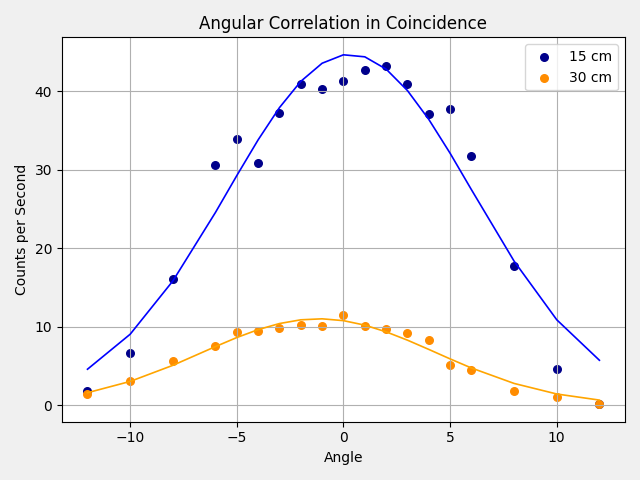
\includegraphics[width=0.45\textwidth]{Figures/coincidence_gauss_fit.png}
    \caption{Data from Table 1 data visualized and fitted with a Gaussian
    function of irrelevant cofidence interval.}
    \label{figure:model1_graph}
\end{figure}
\begin{figure}[H]
    \centering
    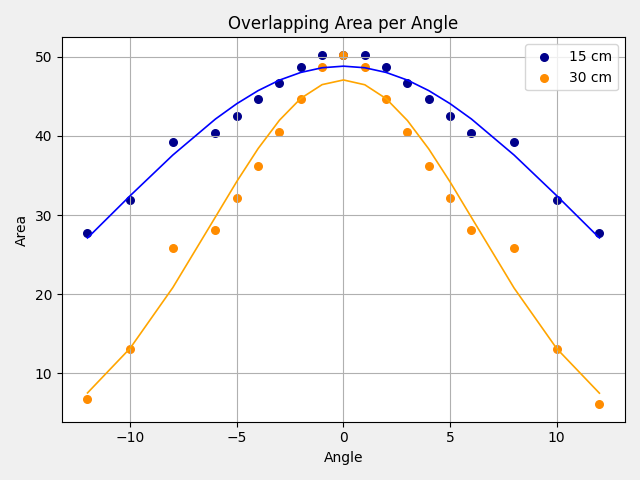
\includegraphics[width=0.45\textwidth]{Figures/overlapping_area_gauss_fit.png}
    \caption{Tables 3 and 4 visualized. The lines simply connect each point and
    do not reflect a line of fit.}
    \label{figure:model2_graph}
\end{figure}
\begin{figure}[H]
    \centering
    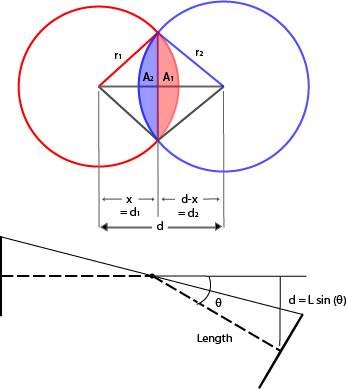
\includegraphics[width=0.45\textwidth]{Figures/geometry.jpg}
    \caption{Set up of the geometry used to derive the correlation between
    overlapping area and angular offset.}
    \label{figure:geometry}
\end{figure}
% Conclusion
\section{Conclusion}
While there are no strong correlations between the two models, there are
similarities in where the maximum of each data set is and the general trend to
decrease as the angle sweeps out. Regardless of having no exact match of fit,
the fact that the two sets of data correlate in the slightest, is enough to
support our hypothesis. The angle between between coincident gammas is was
supported to be 180 degrees.
\end{document}
